\documentclass{article}
\usepackage[utf8]{inputenc}

\usepackage{booktabs}  % for pretty tables

\usepackage{amsmath}   % for math environments
\usepackage{amssymb}   % for special math symbols

\usepackage{tikz}      % for making the desired graphical models
\usetikzlibrary{bayesnet} % for drawing graphical models

\usepackage[margin=1in]{geometry}    % to get 1-inch margins

\title{On the Importance of Modeling\\Unmeasured Confounders in Predictive Inference}
\author{Timothy Brathwaite}
\date{March 21st, 2020}

\begin{document}

\maketitle

\section{Introduction}
\label{sec:intro}
In a general prediction problem, the quantity we want to estimate is $P \left( Y^{*} \mid X^{*}, X, Y \right)$. Algebraically, this can be written using the rules of probability theory as follows.

\begin{equation}
\label{eq:general-prediction}
\begin{aligned}
P \left( Y^{*} \mid X^{*}, X, Y \right) &= \int P \left( Y^{*}, \lambda \mid X^{*}, X, Y \right) \partial \lambda\\
&= \int P \left( Y^{*} \mid X^{*}, X, Y, \lambda \right) P \left( \lambda \mid X^{*}, X, Y \right) \partial \lambda\\
\textrm{where } Y^{*} &= \textrm{The outcome value for a new observation.}\\
X^{*} &= \textrm{The explanatory variables for a new observation.}\\
Y &= \textrm{The historical outcome values.}\\
X &= \textrm{The historical explanatory values.}\\
\lambda &= \textrm{Everything we don't know that affects $X$ and/or $Y$.}\\
\end{aligned}
\end{equation}

At this point, our expression contains two terms. The first term is a model for $Y^{*}$, $P \left( Y^{*} \mid X^{*}, X, Y, \lambda \right)$. The second is a probability for unknown variables $\lambda$, $P \left( \lambda \mid X^{*}, X, Y \right)$. As written, this expression is not useful because we don't know the form of $P \left( \lambda \mid X^{*}, X, Y \right)$. To re-express $P \left( \lambda \mid X^{*}, X, Y \right)$ in terms of quantities we know or can estimate, it is helpful to further specify what $\lambda$ is. In particular, we can decompose $\lambda$ as follows. Either:
\begin{enumerate}
    \item $\lambda = \left( \tau, \theta \right)$ or
    \item $\lambda = \left( \tau, \theta, \Omega \right)$
\end{enumerate}
In these scenarios, $\tau$ represents unknown variables that only affect $X$, $\theta$ represents unknown variables that affect $Y$, and $\Omega$ represents variables that affect both $X$ and $Y$.

Likewise, it is useful to specify the type of relationships that can exist between $X$ and $Y$. We have four types of relationships:
\begin{enumerate}
    \item $X$ causes $Y$
    \item $Y$ causes $X$
    \item $X$ does not cause $Y$ AND $Y$ does not cause $X$
    \item $X$ causes $Y$ AND $Y$ causes $X$.
\end{enumerate}

For the moment, we will ignore case four, because it is a mathematically hard case to deal with and because it is uncommon in most practical cases that I deal with. In most problems I face, $Y$ is an outcome of interest that occurs at time $t$ and $X$ is produced at time $t'$ where $t' < t$, so it is not sensible that $Y$ works backwards in time to cause $X$.

So, combining the three remaining types of relationships between $X$ and $Y$ with the two types of $\lambda$, we have the following 6 graphical models.

\begin{tabular}{lc|c}
\toprule
Case & $\lambda = \left( \tau, \theta \right)$ & $\lambda = \left( \tau, \theta, \Omega \right)$ \\ 
\midrule
(i) & 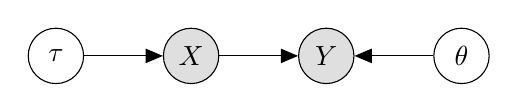
\begin{tikzpicture}
			\node[obs]                               (y) {$Y$};
 			 \node[obs, left=of y]                (x) {$X$};
  
  			 \node[latent,left=of x] (tau) {$\tau$};
  			 \node[latent, right=of y]  (theta) {$\theta$};
  			 
  			 \edge {tau}     {x};
  			 \edge {x}         {y};
  			 \edge {theta}  {y};
		\end{tikzpicture} & 
		
		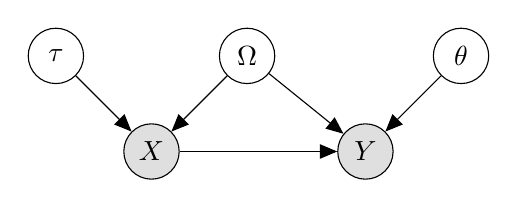
\begin{tikzpicture}
  			% Define nodes
  			\node[obs]                                   (y) {$Y$};
  			\node[obs, left=2cm of y]           (x) {$X$};
 			\node[latent, above left=of x]     (tau) {$\tau$};
  			\node[latent, above right=of y]  (theta) {$\theta$};
 			\node[latent, above right=of x]  (omega) {$\Omega$};

  			% Connect the nodes
 		    \edge {x}                      {y};
  			\edge {tau, omega}     {x};
  			\edge {omega, theta} {y};
		\end{tikzpicture} \\ 
\hline 
(ii) & 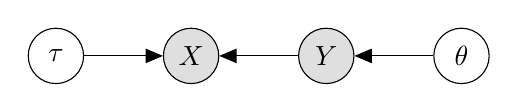
\begin{tikzpicture}
			\node[obs]                               (y) {$Y$};
 			 \node[obs, left=of y]                (x) {$X$};
  
  			 \node[latent,left=of x] (tau) {$\tau$};
  			 \node[latent, right=of y]  (theta) {$\theta$};
  			 
  			 \edge {tau}     {x};
  			 \edge {y}         {x};
  			 \edge {theta}  {y};
		\end{tikzpicture} & 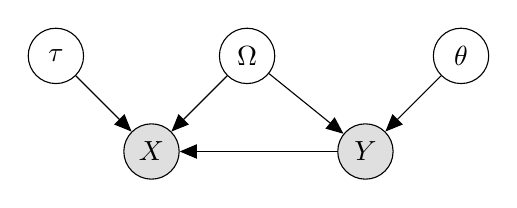
\begin{tikzpicture}

  			% Define nodes
  			\node[obs]                               (y) {$Y$};
  			\node[obs, left=2cm of y]                (x) {$X$};
 			\node[latent, above left=of x] (tau) {$\tau$};
  			\node[latent, above right=of y]  (theta) {$\theta$};
 			\node[latent, above right=of x]  (omega) {$\Omega$};

  			% Connect the nodes
 		    \edge {y}            {x};
  			\edge {tau, omega}   {x};
  			\edge {omega, theta} {y};
		\end{tikzpicture} \\ 
\hline 
(iii) & 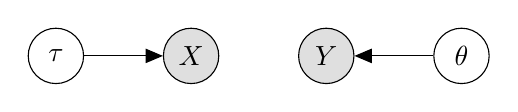
\begin{tikzpicture}
			\node[obs]                               (y) {$Y$};
 			 \node[obs, left=of y]                (x) {$X$};
  
  			 \node[latent,left=of x] (tau) {$\tau$};
  			 \node[latent, right=of y]  (theta) {$\theta$};
  			 
  			 \edge {tau}     {x};
  			 \edge {theta}  {y};
		\end{tikzpicture} & 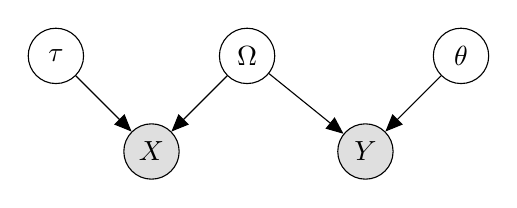
\begin{tikzpicture}

  			% Define nodes
  			\node[obs]                               (y) {$Y$};
  			\node[obs, left=2cm of y]                (x) {$X$};
 			\node[latent, above left=of x] (tau) {$\tau$};
  			\node[latent, above right=of y]  (theta) {$\theta$};
 			\node[latent, above right=of x]  (omega) {$\Omega$};

  			% Connect the nodes
  			\edge {tau, omega}   {x};
  			\edge {omega, theta} {y};
		\end{tikzpicture} \\ 
\bottomrule
\end{tabular} 

\vspace{1cm}
As will be shown in the Section \ref{sec:deriving-known-models}, cases where $\lambda = \left( \tau, \theta \right)$ correspond to ``typical'' supervised learning models. Specifically, cases with $\lambda = \left( \tau, \theta \right)$ and:
\begin{itemize}
    \item $X \rightarrow Y$ correspond to discriminative models (e.g. logistic regression).
    \item $X \leftarrow Y$ correspond to generative models (e.g. naive bayes).
    \item $X \quad \  Y$ (e.g. case iii) correspond to ``constant'' models, where no features are useful for predicting $Y$.
\end{itemize}

Scenarios where unobserved confounding is present, i.e. where $\lambda = \left( \tau, \theta, \Omega \right)$, are not so commonly discussed in machine learning texts.

\section{The Current Scenario:\\A Discriminative Model with Unobserved Confounding}
In particular, the case I want to focus on is depicted by the following graphical model.
\begin{center}
		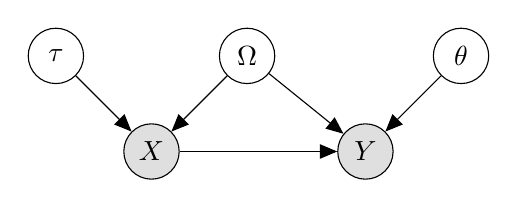
\begin{tikzpicture}
  			% Define nodes
  			\node[obs]                                   (y) {$Y$};
  			\node[obs, left=2cm of y]           (x) {$X$};
 			\node[latent, above left=of x]     (tau) {$\tau$};
  			\node[latent, above right=of y]  (theta) {$\theta$};
 			\node[latent, above right=of x]  (omega) {$\Omega$};

  			% Connect the nodes
 		    \edge {x}                      {y};
  			\edge {tau, omega}     {x};
  			\edge {omega, theta} {y};
		\end{tikzpicture}
\end{center}

In this scenario, there are unmeasured confounders $\Omega$ that cause both $X$ and $Y$, and we also believe that $X \rightarrow Y$. For example, if considering $X$ to be commute travel cost and $Y$ to be transportation mode (e.g. bike, walk, drive, transit), an example of an unobserved confounder might be travel distance if you don't know a user's exact home address. The travel distance will cause one's travel cost and may cause one's travel mode as well (e.g. if a person doesn't want to walk a long distance).

Let's see how we can calculate $P \left( Y^{*} \mid X^{*}, X, Y \right)$ in this scenario. Using Equation \ref{eq:general-prediction} and the factorization of $P \left( X^{*}, X, Y \mid \lambda \right)$ implied by the directed acyclic graph (DAG) above, we can continue writing

\begin{equation}
\label{eq:prediction-simplified-1}
\begin{aligned}
P \left( Y^{*} \mid X^{*}, X, Y \right) &=  \int P \left( Y^{*} \mid X^{*}, X, Y, \lambda \right) P \left( \lambda \mid X^{*}, X, Y \right) \partial \lambda\\
&= \int P \left( Y^{*} \mid X^{*}, \lambda \right) P \left( \lambda \mid X^{*}, X, Y \right) \partial \lambda\\
&= \int P \left( Y^{*} \mid X^{*}, \Omega, \theta \right) P \left( \lambda \mid X^{*}, X, Y \right) \partial \lambda
\end{aligned}
\end{equation}

Next, the term $P \left( \lambda \mid X^{*}, X, Y \right)$ can be calculated using Bayes' Rule and by (again) relying on the factorization from the DAG above.
\begin{equation}
\label{eq:lambda-given-everything}
\begin{aligned}
P \left( \lambda \mid X^{*}, X, Y \right) &= \frac{P \left( X^{*}, X, Y \mid \lambda \right) P \left( \lambda \right)}{P \left( X^{*}, X, Y \right)}\\
&= \frac{P \left( X^{*} \mid \lambda \right) P \left( X, Y \mid \lambda \right) P \left( \lambda \right)}{P \left( X^{*}, X, Y \right)}\\
&= \frac{P \left( X^{*} \mid \lambda \right) P \left( Y \mid X, \lambda \right) P \left( X \mid \lambda \right) P \left( \lambda \right)}{P \left( X^{*}, X, Y \right)}\\
&= \frac{P \left( X^{*} \mid \tau, \Omega \right) P \left( Y \mid X, \theta, \Omega \right) P \left( X \mid \tau, \Omega \right) P \left( \lambda \right)}{P \left( X^{*}, X, Y \right)}
\end{aligned}
\end{equation}

Substituting Equation \ref{eq:lambda-given-everything} into Equation \ref{eq:prediction-simplified-1}, we get the following expression.
\begin{equation}
\label{eq:prediction-simplified-2}
\begin{aligned}
P \left( Y^{*} \mid X^{*}, X, Y \right) &= \int \left[ \frac{P \left( Y^{*} \mid X^{*}, \theta, \Omega \right) P \left( X^{*} \mid \tau, \Omega \right) P \left( Y \mid X, \theta, \Omega \right) P \left( X \mid \tau, \Omega \right) P \left( \lambda \right)}{P \left( X^{*}, X, Y \right)} \right] \partial \lambda\\
&= \frac{ \int P \left( Y^{*} \mid X^{*}, \theta, \Omega \right) P \left( X^{*} \mid \tau, \Omega \right) P \left( Y \mid X, \theta, \Omega \right) P \left( X \mid \tau, \Omega \right) P \left( \lambda \right) \partial \lambda }{P \left( X^{*}, X, Y \right)}\\
&= \dfrac{ \int \left[ \dfrac{P \left( Y^{*} \mid X^{*}, \theta, \Omega \right) P \left( X^{*} \mid \tau, \Omega \right) P \left( Y \mid X, \theta, \Omega \right) P \left( X \mid \tau, \Omega \right) P \left( \lambda \right)}{P \left( X, Y \right)} \right] \partial \lambda }{\dfrac{P \left( X^{*}, X, Y \right)}{P \left( X, Y \right)}}\\
&= \frac{ \int P \left( Y^{*} \mid X^{*}, \theta, \Omega \right) P \left( X^{*} \mid \tau, \Omega \right) P \left( \lambda \mid X, Y \right) \partial \lambda }{\dfrac{P \left( X^{*}, X, Y \right)}{P \left( X, Y \right)}}\\
&= \frac{ \int P \left( Y^{*} \mid X^{*}, \theta, \Omega \right) P \left( X^{*} \mid \tau, \Omega \right) P \left( \lambda \mid X, Y \right) \partial \lambda }{P \left( X^{*} \mid X, Y \right)}\\
&\propto  \int P \left( Y^{*} \mid X^{*}, \theta, \Omega \right) P \left( X^{*} \mid \tau, \Omega \right) P \left( \lambda \mid X, Y \right) \partial \lambda\\
&\approx \frac{1}{M} \sum _{i=1} ^M P \left( Y^{*} \mid X^{*}, \theta_i, \Omega_i \right) P \left( X^{*} \mid \tau_i, \Omega_i \right)\\
\textrm{where } M &= \textrm{The number of samples from $P \left( \lambda \mid X, Y \right)$}\\
\lambda_i &= \left( \tau_i, \theta_i, \Omega_i \right) = \textrm{A singe sample from $P \left( \lambda \mid X, Y \right)$}\\
P \left( \lambda \mid X, Y \right) &= \frac{P \left( Y \mid X, \theta, \Omega \right) P \left( X \mid \tau, \Omega \right) P \left( \lambda \right)}{P \left( X, Y \right)}
\end{aligned}
\end{equation}

The reasoning above suggests that at prediction time, we should use a Monte Carlo estimate of the joint probability of $\left( X^{*}, Y^{*} \right)$. We can then normalize across $Y^{*}$ to get a probability in [0, 1].

During training, we should estimate the posterior distribution $P \left( \lambda \mid X, Y \right)$. Given that $\Omega$ is expected to have at least one component per individual and we will only have one or at most a few observations per person in our dataset, we will likely not be in a world where the posterior distribution has concentrated on a single point. Accordingly, it would be best to estimate the entire posterior distribution since there may be wide uncertainty in our posterior beliefs about the value of the unmeasured confounders for some of the observations. However, if one persists in relying on point estimates, one can estimate the maximum a-posterior (MAP) point, which selects $\lambda$ to maximize the numerator: $P \left( Y \mid X, \theta, \Omega \right) P \left( X \mid \tau, \Omega \right) P \left( \lambda \right)$.

\section{Deriving Known Models}
\label{sec:deriving-known-models}
At the end of Section \ref{sec:intro}, I stated that the situation where $\lambda = \left( \tau, \theta \right)$ corresponded to most typically used models such as discriminative and generative models. Below I'll provide a proof of these two points.

\subsection{Discriminative Models}
Discriminative models can be derived from the following graphical model where $\lambda = \left( \tau, \theta \right)$:\newline
\begin{center}
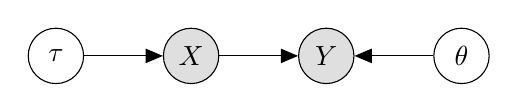
\begin{tikzpicture}
		\node[obs]                        (y) {$Y$};
 		\node[obs, left=of y]        (x) {$X$};
  
  		\node[latent,left=of x]     (tau) {$\tau$};
  		\node[latent, right=of y]  (theta) {$\theta$};
  			 
  		\edge {tau}     {x};
  		\edge {x}         {y};
  		\edge {theta}  {y};
\end{tikzpicture}
\end{center}
The derivation begins with Equation \ref{eq:general-prediction} and, using the DAG above, proceeds as follows.
\begin{equation}
\label{eq:discriminative-prediction}
\begin{aligned}
P \left( Y^{*} \mid X^{*}, X, Y \right) &= \int P \left( Y^{*} \mid X^{*}, X, Y, \lambda \right) P \left( \lambda \mid X^{*}, X, Y \right) \partial \lambda\\
&= \int P \left( Y^{*} \mid X^{*}, \lambda \right) P \left( \lambda \mid X^{*}, X, Y \right) \partial \lambda\\
&= \int P \left( Y^{*} \mid X^{*}, \lambda \right) \frac{P \left( X^{*}, X, Y \mid \lambda \right) P \left( \lambda \right)}{P \left( X^{*}, X, Y \right)} \partial \lambda\\
&= \int \int P \left( Y^{*} \mid X^{*}, \tau, \theta \right) \frac{P \left( X^{*}, X, Y \mid \tau, \theta \right) P \left( \tau, \theta \right)}{P \left( X^{*}, X, Y \right)} \partial \tau \partial \theta\\
&= \int \int P \left( Y^{*} \mid X^{*}, \theta \right) \frac{P \left( X^{*} \mid \tau \right) P\left( X, Y \mid \tau, \theta \right) P \left( \tau, \theta \right)}{P \left( X^{*}, X, Y \right)} \partial \tau \partial \theta\\
&= \int \int P \left( Y^{*} \mid X^{*}, \theta \right) \frac{P \left( X^{*} \mid \tau \right) P \left( Y \mid X, \theta \right) P\left( X \mid \tau \right) P \left( \tau \right) P\left( \theta \right)}{P \left( X^{*}, X, Y \right)} \partial \tau \partial \theta\\
&= \int P \left( Y^{*} \mid X^{*}, \theta \right) P \left( Y \mid X, \theta \right) P\left( \theta \right) \partial \theta \int \frac{P \left( X^{*} \mid \tau \right) P\left( X \mid \tau \right) P \left( \tau \right)}{P \left( X^{*}, X, Y \right)} \partial \tau\\
&= \frac{1}{P \left( X^{*}, X, Y \right)} \int P \left( Y^{*} \mid X^{*}, \theta \right) P \left( Y \mid X, \theta \right) P\left( \theta \right) \partial \theta \int P \left( X^{*}, X, \tau \right) \partial \tau\\
&= \frac{P \left( X^{*}, X \right)}{P \left( X^{*}, X, Y \right)} \int P \left( Y^{*} \mid X^{*}, \theta \right) P \left( Y \mid X, \theta \right) P\left( \theta \right) \partial \theta \\
&= \dfrac{P \left( X^{*}, X \right)}{\dfrac{P \left( X^{*}, X, Y \right)}{P \left( X, Y \right)}} \int P \left( Y^{*} \mid X^{*}, \theta \right) \dfrac{P \left( Y \mid X, \theta \right) P\left( \theta \right)}{P \left( X, Y \right)} \partial \theta\\
&= \dfrac{\dfrac{P \left( X^{*}, X \right)}{P \left( X \right)}}{\dfrac{P \left( X^{*}, X, Y \right)}{P \left( X, Y \right)}} \int P \left( Y^{*} \mid X^{*}, \theta \right) \dfrac{P \left( Y \mid X, \theta \right) P \left( X \right) P\left( \theta \right)}{P \left( X, Y \right)} \partial \theta\\
&= \dfrac{\dfrac{P \left( X^{*}, X \right)}{P \left( X \right)}}{\dfrac{P \left( X^{*}, X, Y \right)}{P \left( X, Y \right)}} \int P \left( Y^{*} \mid X^{*}, \theta \right) \dfrac{P \left( Y \mid X, \theta \right) P \left( X \mid \theta \right) P\left( \theta \right)}{P \left( X, Y \right)} \partial \theta\\
&= \frac{P \left( X^{*} \mid X \right)}{P \left( X^{*} \mid X, Y \right)} \int P \left( Y^{*} \mid X^{*}, \theta \right) \frac{P \left( Y, X, \theta \right)}{P \left( X, Y \right)} \partial \theta\\
&= \frac{P \left( X^{*} \mid X \right)}{P \left( X^{*} \mid X, Y \right)} \int P \left( Y^{*} \mid X^{*}, \theta \right) P \left( \theta \mid X, Y \right) \partial \theta\\
&=\int P \left( Y^{*} \mid X^{*}, \theta \right) P \left( \theta \mid X, Y \right) \partial \theta
\end{aligned}
\end{equation}

The last line in Equation \ref{eq:discriminative-prediction} follows from the following equality:
\begin{equation}
\begin{aligned}
\frac{P \left( X^{*} \mid X \right)}{P \left( X^{*} \mid X, Y \right)} &= \frac{\int P \left( X^{*}, \tau \mid X \right) \partial \tau}{\int P \left( X^{*}, \tau \mid X, Y \right) \partial \tau}\\
&= \frac{\int P \left( X^{*} \mid \tau, X \right) P \left( \tau \mid X \right) \partial \tau}{ \int P \left( X^{*} \mid \tau, X, Y \right) P \left( \tau \mid X, Y \right) \partial \tau}\\
&= \frac{\int P \left( X^{*} \mid \tau \right) P \left( \tau \mid X \right) \partial \tau}{\int P \left( X^{*} \mid \tau \right) P \left( \tau \mid X\right) \partial \tau}\\
&= 1
\end{aligned}
\end{equation}
Moreover, the last line in Equation \ref{eq:discriminative-prediction} justifies the discriminative learning technique of (1) building a model for $Y$ as a function of $X$ and $\theta$, and (2) taking the expectation of that model's outputs with respect to the posterior distribution of $\theta$. By Equation \ref{eq:discriminative-prediction}, no other models are required. In particular, no models of $X$ are needed. Note that this contrasts the equivalent scenario with unobserved confounding. There, one needs both a model for $Y$ AND a model for $X$.

\subsection{Generative Models}
In this section, I'll show how generative models come from the following graphical model:
\newline
\begin{center}
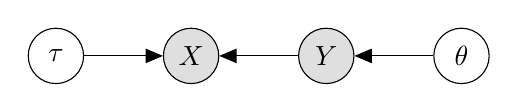
\begin{tikzpicture}
		\node[obs]                        (y) {$Y$};
 		\node[obs, left=of y]        (x) {$X$};
  
  		\node[latent,left=of x]     (tau) {$\tau$};
  		\node[latent, right=of y]  (theta) {$\theta$};
  			 
  		\edge {tau}     {x};
  		\edge {y}         {x};
  		\edge {theta}  {y};
\end{tikzpicture}
\end{center}
First, it is important to note that this graphical model admits the following factorization of the joint probability $P \left( X, Y, \tau, \theta \right)$: $\left\lbrace P\left( X \mid \tau, Y \right), P \left( Y \mid \theta \right), P \left( \tau \right), P \left( \theta \right) \right\rbrace$. As a result, all of our probabilistic expressions for these variables should be written in terms of these basic elements. This requires that we re-express the following probability from Equation \ref{eq:general-prediction} as follows:
\begin{equation}
\label{eq:desired-generative-prediction}
\begin{aligned}
P \left( Y^{*} \mid X^{*}, X, Y, \lambda \right) &= P \left( Y^{*} \mid X^{*}, \lambda \right)\\
&= \frac{P \left( X^{*}, Y^{*} \mid \lambda \right)}{P \left( X^{*} \mid \lambda \right)}\\
&= \frac{P \left( X^{*} \mid Y^{*}, \lambda \right) P \left( Y^{*} \mid \lambda \right)}{ P \left( X^{*} \mid \lambda \right) }\\
&= \frac{P \left( X^{*} \mid Y^{*}, \tau \right) P \left( Y^{*} \mid \theta \right)}{ P \left( X^{*} \mid \tau, \theta \right) }\\
\end{aligned}
\end{equation}

Similarly, we will need the following re-expression:
\begin{equation}
\label{eq:auxillary-generative}
\begin{aligned}
P \left( X^{*}, X, Y \mid \lambda \right) &= P \left( X^{*} \mid X, Y, \lambda \right) P \left( X, Y \mid \lambda \right)\\
&= P \left( X^{*} \mid \lambda \right) P \left( X, Y \mid \lambda \right)\\
&= P \left( X^{*} \mid \tau, \theta \right) P \left( X, Y \mid \tau, \theta \right)\\
&= P \left( X^{*} \mid \tau, \theta \right) P \left( X \mid Y, \tau, \theta \right) P \left( Y \mid \tau, \theta \right)\\
&= P \left( X^{*} \mid \tau, \theta \right) P \left( X \mid Y, \tau \right) P \left( Y \mid \theta \right)
\end{aligned}
\end{equation}
With these expressions, we can now return to Equation \ref{eq:general-prediction} and proceed in the following manner:
\begin{equation}
\label{eq:generative-prediction}
\begin{aligned}
P \left( Y^{*} \mid X^{*}, X, Y \right) &= \int P \left( Y^{*} \mid X^{*}, X, Y, \lambda \right) P \left( \lambda \mid X^{*}, X, Y \right) \partial \lambda\\
&= \int \frac{P \left( X^{*} \mid Y^{*}, \tau \right) P \left( Y^{*} \mid \theta \right)}{ P \left( X^{*} \mid \tau, \theta \right) } P \left( \lambda \mid X^{*}, X, Y \right) \partial \lambda\\
&= \int \frac{P \left( X^{*} \mid Y^{*}, \tau \right) P \left( Y^{*} \mid \theta \right)}{ P \left( X^{*} \mid \tau, \theta \right)} \frac{P \left( X^{*}, X, Y \mid \lambda \right) P \left( \lambda \right)}{P \left( X^{*}, X, Y \right)} \partial \lambda\\
&= \int \frac{P \left( X^{*} \mid Y^{*}, \tau \right) P \left( Y^{*} \mid \theta \right)}{ P \left( X^{*} \mid \tau, \theta \right) } \frac{P \left( X^{*} \mid \tau, \theta \right) P \left( X, Y \mid \tau, \theta \right) P \left( \lambda \right)}{P \left( X^{*}, X, Y \right)} \partial \lambda\\
&= \int P \left( X^{*} \mid Y^{*}, \tau \right) P \left( Y^{*} \mid \theta \right) \frac{ P \left( X, Y \mid \tau, \theta \right) P \left( \lambda \right)}{P \left( X^{*}, X, Y \right)} \partial \lambda\\
&= \int P \left( X^{*} \mid Y^{*}, \tau \right) P \left( Y^{*} \mid \theta \right) \dfrac{ \dfrac{P \left( X, Y \mid \tau, \theta \right) P \left( \lambda \right)}{P \left( X, Y \right)}}{\dfrac{P \left( X^{*}, X, Y \right)}{P \left( X, Y \right)}} \partial \lambda\\
&= \int P \left( X^{*} \mid Y^{*}, \tau \right) P \left( Y^{*} \mid \theta \right) \frac{ P \left( \tau, \theta \mid X, Y \right) }{P \left( X^{*} \mid X, Y \right)} \partial \lambda\\
&\propto \int P \left( X^{*} \mid Y^{*}, \tau \right) P \left( Y^{*} \mid \theta \right) P \left( \tau, \theta \mid X, Y \right) \partial \lambda\\
\textrm{where } P \left( \tau, \theta \mid X, Y \right) &= \frac{P \left( X, Y \mid \tau, \theta \right)}{P \left( X, Y \right)}\\
&= \frac{P \left( X \mid Y, \tau \right) P \left( Y \mid \theta \right) P \left( \lambda \right)}{P \left( X, Y \right)}
\end{aligned}
\end{equation}
The last three lines of Equation \ref{eq:generative-prediction} justify the  typical generative model. First, models are built for $P \left( X \mid Y, \tau \right)$ and $P \left( Y \mid \theta \right)$. From these two models we can estimate the posterior distribution of $\lambda$: $P \left( \tau, \theta \mid X, Y \right)$. Secondly, given samples from $P \left( \tau, \theta \mid X, Y \right)$, we can use the two aforementioned models to construct a Monte Carlo estimate of $P \left( X^{*}, Y^{*} \mid X, Y \right)$. Finally, we can normalize across $Y^{*}$ to calculate $P \left( Y^{*} \mid X^{*}, X, Y \right)$.

Here, as in the case of a discriminative model with unobserved confounding, we need both a model of $X$ AND a model of $Y$.

\section{A Generative Model with Unobserved Confounding}
This case is conceptually very similar to the generative model that was just presented. As a result I will proceed by analogy and provide any missing derivations only as requested by others.

First, the graphical model that depicts this scenario is
\begin{center}
		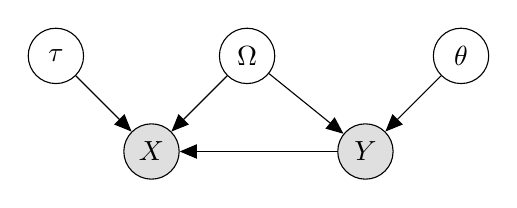
\begin{tikzpicture}
  			% Define nodes
  			\node[obs]                                   (y) {$Y$};
  			\node[obs, left=2cm of y]           (x) {$X$};
 			\node[latent, above left=of x]     (tau) {$\tau$};
  			\node[latent, above right=of y]  (theta) {$\theta$};
 			\node[latent, above right=of x]  (omega) {$\Omega$};

  			% Connect the nodes
 		    \edge {y}                      {x};
  			\edge {tau, omega}     {x};
  			\edge {omega, theta} {y};
		\end{tikzpicture}
\end{center}

Secondly, the desired predictive distribution is:
\begin{equation}
\label{eq:confounded-generative-prediction}
\begin{aligned}
P \left( Y^{*} \mid X^{*}, X, Y \right) &= \int P \left( Y^{*} \mid X^{*}, X, Y, \lambda \right) P \left( \lambda \mid X^{*}, X, Y \right) \partial \lambda\\
&= \int \frac{P \left( X^{*} \mid Y^{*}, \tau, \Omega \right) P \left( Y^{*} \mid \theta, \Omega \right)}{ P \left( X^{*} \mid \tau, \theta, \Omega \right) } P \left( \lambda \mid X^{*}, X, Y \right) \partial \lambda\\
&= \int \frac{P \left( X^{*} \mid Y^{*}, \tau, \Omega \right) P \left( Y^{*} \mid \theta, \Omega \right)}{ P \left( X^{*} \mid \tau, \theta, \Omega \right)} \frac{P \left( X^{*}, X, Y \mid \lambda \right) P \left( \lambda \right)}{P \left( X^{*}, X, Y \right)} \partial \lambda\\
&= \int \frac{P \left( X^{*} \mid Y^{*}, \tau, \Omega \right) P \left( Y^{*} \mid \theta, \Omega \right)}{ P \left( X^{*} \mid \tau, \theta, \Omega \right) } \frac{P \left( X^{*} \mid \tau, \theta, \Omega \right) P \left( X, Y \mid \tau, \theta, \Omega \right) P \left( \lambda \right)}{P \left( X^{*}, X, Y \right)} \partial \lambda\\
&= \int P \left( X^{*} \mid Y^{*}, \tau, \Omega \right) P \left( Y^{*} \mid \theta, \Omega \right) \frac{ P \left( X, Y \mid \tau, \theta, \Omega \right) P \left( \lambda \right)}{P \left( X^{*}, X, Y \right)} \partial \lambda\\
&= \int P \left( X^{*} \mid Y^{*}, \tau, \Omega \right) P \left( Y^{*} \mid \theta, \Omega \right) \dfrac{ \dfrac{P \left( X, Y \mid \tau, \theta, \Omega \right) P \left( \lambda \right)}{P \left( X, Y \right)}}{\dfrac{P \left( X^{*}, X, Y \right)}{P \left( X, Y \right)}} \partial \lambda\\
&= \int P \left( X^{*} \mid Y^{*}, \tau, \Omega \right) P \left( Y^{*} \mid \theta, \Omega \right) \frac{ P \left( \tau, \theta, \Omega \mid X, Y \right) }{P \left( X^{*} \mid X, Y \right)} \partial \lambda\\
&\propto \int P \left( X^{*} \mid Y^{*}, \tau, \Omega \right) P \left( Y^{*} \mid \theta, \Omega \right) P \left( \tau, \theta, \Omega \mid X, Y \right) \partial \lambda\\
\textrm{where } P \left( \tau, \theta, \Omega \mid X, Y \right) &= \frac{P \left( X, Y \mid \tau, \theta, \Omega \right)}{P \left( X, Y \right)}\\
&= \frac{P \left( X \mid Y, \tau, \Omega \right) P \left( Y \mid \theta, \Omega \right) P \left( \lambda \right)}{P \left( X, Y \right)}
\end{aligned}
\end{equation}
As shown by the last three lines of Equation \ref{eq:confounded-generative-prediction} versus the last three lines of Equation \ref{eq:generative-prediction}, there is little mathematical difference between generative models with and without unobserved confounding. Moreover, the prediction equation for a generative model with confounding and a discriminative model with confounding are symmetric: switch $X$ and $Y$ and switch $\tau$ and $\theta$.

\end{document}
